\documentclass[10pt]{article}\usepackage[]{graphicx}\usepackage[]{color}
%% maxwidth is the original width if it is less than linewidth
%% otherwise use linewidth (to make sure the graphics do not exceed the margin)
\makeatletter
\def\maxwidth{ %
  \ifdim\Gin@nat@width>\linewidth
    \linewidth
  \else
    \Gin@nat@width
  \fi
}
\makeatother

\definecolor{fgcolor}{rgb}{0.345, 0.345, 0.345}
\newcommand{\hlnum}[1]{\textcolor[rgb]{0.686,0.059,0.569}{#1}}%
\newcommand{\hlstr}[1]{\textcolor[rgb]{0.192,0.494,0.8}{#1}}%
\newcommand{\hlcom}[1]{\textcolor[rgb]{0.678,0.584,0.686}{\textit{#1}}}%
\newcommand{\hlopt}[1]{\textcolor[rgb]{0,0,0}{#1}}%
\newcommand{\hlstd}[1]{\textcolor[rgb]{0.345,0.345,0.345}{#1}}%
\newcommand{\hlkwa}[1]{\textcolor[rgb]{0.161,0.373,0.58}{\textbf{#1}}}%
\newcommand{\hlkwb}[1]{\textcolor[rgb]{0.69,0.353,0.396}{#1}}%
\newcommand{\hlkwc}[1]{\textcolor[rgb]{0.333,0.667,0.333}{#1}}%
\newcommand{\hlkwd}[1]{\textcolor[rgb]{0.737,0.353,0.396}{\textbf{#1}}}%
\let\hlipl\hlkwb

\usepackage{framed}
\makeatletter
\newenvironment{kframe}{%
 \def\at@end@of@kframe{}%
 \ifinner\ifhmode%
  \def\at@end@of@kframe{\end{minipage}}%
  \begin{minipage}{\columnwidth}%
 \fi\fi%
 \def\FrameCommand##1{\hskip\@totalleftmargin \hskip-\fboxsep
 \colorbox{shadecolor}{##1}\hskip-\fboxsep
     % There is no \\@totalrightmargin, so:
     \hskip-\linewidth \hskip-\@totalleftmargin \hskip\columnwidth}%
 \MakeFramed {\advance\hsize-\width
   \@totalleftmargin\z@ \linewidth\hsize
   \@setminipage}}%
 {\par\unskip\endMakeFramed%
 \at@end@of@kframe}
\makeatother

\definecolor{shadecolor}{rgb}{.97, .97, .97}
\definecolor{messagecolor}{rgb}{0, 0, 0}
\definecolor{warningcolor}{rgb}{1, 0, 1}
\definecolor{errorcolor}{rgb}{1, 0, 0}
\newenvironment{knitrout}{}{} % an empty environment to be redefined in TeX

\usepackage{alltt}
\usepackage{amssymb, amsmath, amsthm, verbatim, layout, setspace, graphicx, float, geometry}
\usepackage{booktabs}

\newcommand{\textnote}[1]{\textbf{\textit{#1}}}
\newcommand{\code}[1]{\textbf{\textit{#1}}}
\newcommand{\grad}{\nabla}

% ------ layout ------
\IfFileExists{upquote.sty}{\usepackage{upquote}}{}
\begin{document}
\title{Linear Regression}
\author{Jeremy Oldfather}
\maketitle



\section*{Review}

\subsection*{What is linear regression?}

Start with a line.

\begin{align}
y &= mx + b \label{line}
\end{align}


We know what this looks like visually. The line crosses the y-axis at the height of $b$ (intercept) and for each unit we move left or right, we move up or down by $m$ (slope) units. For example, with $b=10$ and $m=.7$, we get the following line:

\begin{knitrout}\small
\definecolor{shadecolor}{rgb}{0.969, 0.969, 0.969}\color{fgcolor}\begin{kframe}
\begin{alltt}
\hlstd{b}\hlkwb{<-}\hlnum{10}
\hlstd{m}\hlkwb{<-}\hlnum{.7}
\hlstd{x}\hlkwb{<-}\hlnum{0}\hlopt{:}\hlnum{50}
\hlstd{y}\hlkwb{<-}\hlstd{m}\hlopt{*}\hlstd{x} \hlopt{+} \hlstd{b}
\hlkwd{qplot}\hlstd{(x,y,}\hlkwc{geom}\hlstd{=}\hlstr{"line"}\hlstd{)}
\end{alltt}
\end{kframe}

{\centering 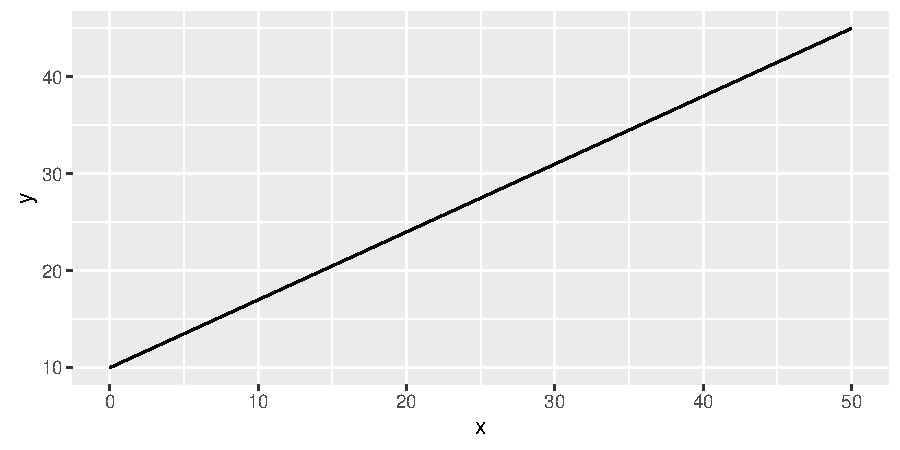
\includegraphics[width=\maxwidth]{figure/simple_line-1} 

}



\end{knitrout}

Since the line has two parameters, $m$ and $b$, we could take any {\bf two} distinct points, draw a line between them, and solve for the parameters. If we only have {\bf one} point, we could draw infinitely many lines through the point.

Let's take this idea to some data. I have some data on the sales of DC properties. We can conceptualize each property as a point. Here is the \code{sale\_price} and \code{living\_sqft} of the first two properties. 

\begin{knitrout}\small
\definecolor{shadecolor}{rgb}{0.969, 0.969, 0.969}\color{fgcolor}\begin{kframe}
\begin{alltt}
\hlcom{# see: https://github.com/theoldfather/DC_Properties}
\hlstd{sales}\hlkwb{<-}\hlkwd{read_csv}\hlstd{(}\hlstr{"~/Projects/DC_Properties/data/sales_clean.csv"}\hlstd{)}
\hlstd{features}\hlkwb{<-}\hlkwd{read_csv}\hlstd{(}\hlstr{"~/Projects/DC_Properties/data/features_clean.csv"}\hlstd{)}
\hlstd{details}\hlkwb{<-}\hlkwd{read_csv}\hlstd{(}\hlstr{"~/Projects/DC_Properties/data/details_clean.csv"}\hlstd{)}
\end{alltt}
\end{kframe}
\end{knitrout}
\begin{knitrout}\small
\definecolor{shadecolor}{rgb}{0.969, 0.969, 0.969}\color{fgcolor}\begin{kframe}
\begin{alltt}
\hlstd{d}\hlkwb{<-}\hlstd{sales} \hlopt
  \hlkwd{filter}\hlstd{(sale_price}\hlopt{>}\hlnum{0}\hlstd{)} \hlopt
  \hlkwd{left_join}\hlstd{(features,}\hlkwc{by}\hlstd{=}\hlstr{"ssl"}\hlstd{)} \hlopt
  \hlkwd{filter}\hlstd{(}\hlopt{!}\hlkwd{is.na}\hlstd{(living_sqft)} \hlopt{&} \hlstd{living_sqft}\hlopt{>}\hlnum{0}\hlstd{)} \hlopt
  \hlkwd{select}\hlstd{(sale_price,living_sqft)}
\hlkwd{head}\hlstd{(d,}\hlnum{2}\hlstd{)} \hlopt \hlkwd{data.frame}\hlstd{()}
\end{alltt}
\begin{verbatim}
##   sale_price living_sqft
## 1     200000        1505
## 2     650000        1281
\end{verbatim}
\end{kframe}
\end{knitrout}

Plotting these two points, we get the following scatterplot.

\begin{knitrout}\small
\definecolor{shadecolor}{rgb}{0.969, 0.969, 0.969}\color{fgcolor}\begin{kframe}
\begin{alltt}
\hlkwd{ggplot}\hlstd{(d[}\hlnum{1}\hlopt{:}\hlnum{2}\hlstd{,],}\hlkwd{aes}\hlstd{(}\hlkwc{x}\hlstd{=living_sqft,}\hlkwc{y}\hlstd{=sale_price))} \hlopt{+} \hlkwd{geom_point}\hlstd{()}
\end{alltt}
\end{kframe}

{\centering 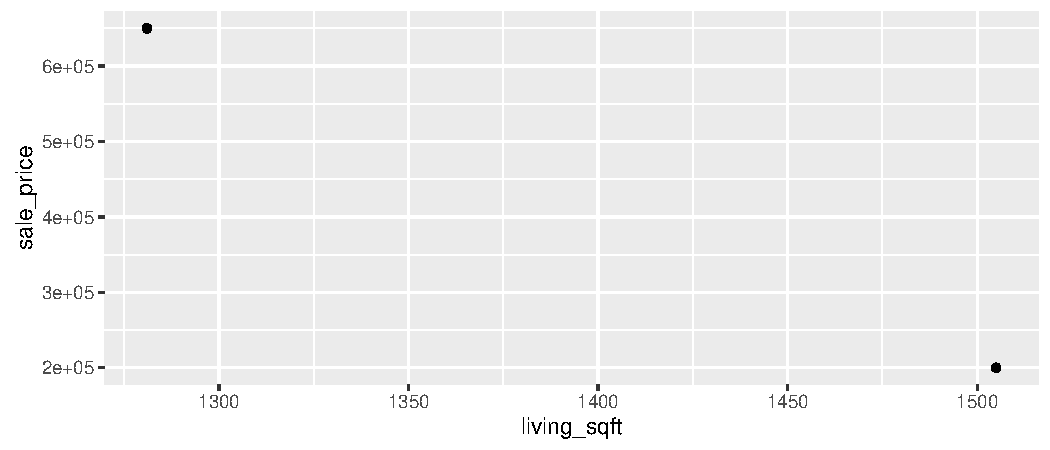
\includegraphics[width=\maxwidth]{figure/plot2-1} 

}



\end{knitrout}

We could draw a segment between the lines by changing \code{geom\_point()} to \code{geom\_line()}, but let's do it by finding the slope and intercept, and then plotting the line through the points.

If we subscript equation \ref{line} with $i$ to represent each observation, we can write it in a condensed notation as

\begin{align}
y_i &= m x_i + b \label{line_general}
\end{align}

and then expand it for $i \in \{1,2\}$.

\begin{align}
y_1 &= m x_1 + b \\
y_2 &= m x_2 + b
\end{align}

Solving for $m$ and $b$ we get

\begin{align}
m = \frac{y_2 - y_1}{x_2-x_1} \label{solution_slope} \\
b = y_1 - mx_1 \label{solution_intercept}
\end{align}

\begin{knitrout}\small
\definecolor{shadecolor}{rgb}{0.969, 0.969, 0.969}\color{fgcolor}\begin{kframe}
\begin{alltt}
\hlstd{fit_line}\hlkwb{<-}\hlkwa{function}\hlstd{(}\hlkwc{y}\hlstd{,}\hlkwc{x}\hlstd{)\{}
  \hlstd{m} \hlkwb{<-} \hlstd{(y[}\hlnum{2}\hlstd{]}\hlopt{-}\hlstd{y[}\hlnum{1}\hlstd{])}\hlopt{/}\hlstd{(x[}\hlnum{2}\hlstd{]}\hlopt{-}\hlstd{x[}\hlnum{1}\hlstd{])}
  \hlstd{b} \hlkwb{<-} \hlstd{y[}\hlnum{1}\hlstd{]} \hlopt{-} \hlstd{m}\hlopt{*}\hlstd{x[}\hlnum{1}\hlstd{]}
  \hlkwd{return}\hlstd{(}\hlkwd{c}\hlstd{(b,m))}
\hlstd{\}}
\hlstd{beta}\hlkwb{<-}\hlkwd{fit_line}\hlstd{(d}\hlopt{$}\hlstd{sale_price[}\hlnum{1}\hlopt{:}\hlnum{2}\hlstd{],d}\hlopt{$}\hlstd{living_sqft[}\hlnum{1}\hlopt{:}\hlnum{2}\hlstd{])}
\hlkwd{ggplot}\hlstd{(d[}\hlnum{1}\hlopt{:}\hlnum{2}\hlstd{,],}\hlkwd{aes}\hlstd{(}\hlkwc{x}\hlstd{=living_sqft,}\hlkwc{y}\hlstd{=sale_price))} \hlopt{+}
  \hlkwd{geom_point}\hlstd{()} \hlopt{+} \hlkwd{geom_abline}\hlstd{(}\hlkwc{intercept}\hlstd{=beta[}\hlnum{1}\hlstd{],}\hlkwc{slope}\hlstd{=beta[}\hlnum{2}\hlstd{])}
\end{alltt}
\end{kframe}

{\centering 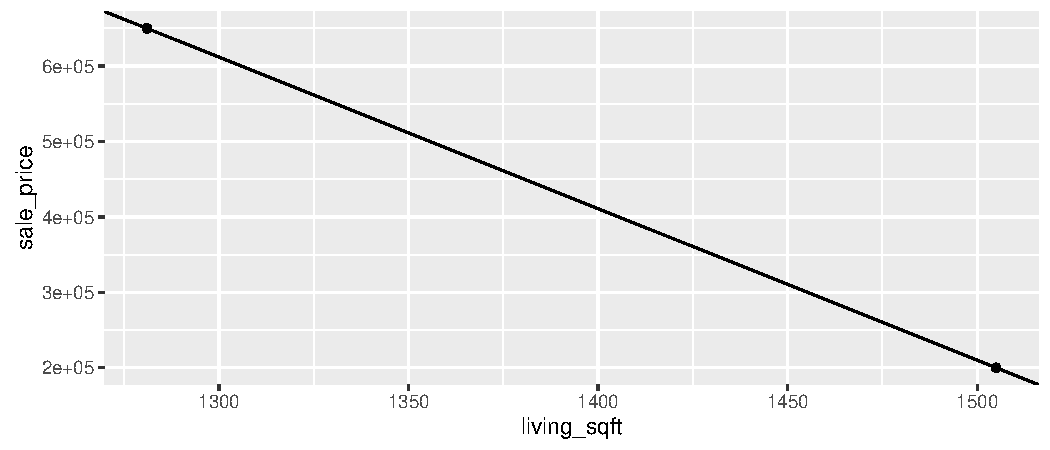
\includegraphics[width=\maxwidth]{figure/fit_line-1} 

}



\end{knitrout}

Do you believe this is an accurate model of the relationship between sales price and the living area of a home? $b=\ensuremath{3.2234375\times 10^{6}}$ implies that a house with no space would be worth \$3 million. And $m=\ensuremath{-2008.9285714}$ implies that increasing the living area of a home by 1 sqft would decrease its values by \$2,008. 

Thankfully, we have data on more than two homes. But what does it mean to draw a line through {\bf more than two} points? We know our model above is very bad---so not every point will fall on the same line.

Here is the rest of our data plotted on log-log scale (we will talk about log-log scale later).

\begin{knitrout}\small
\definecolor{shadecolor}{rgb}{0.969, 0.969, 0.969}\color{fgcolor}\begin{kframe}
\begin{alltt}
\hlkwd{ggplot}\hlstd{(d,}\hlkwd{aes}\hlstd{(}\hlkwc{x}\hlstd{=living_sqft,}\hlkwc{y}\hlstd{=sale_price))} \hlopt{+}
  \hlkwd{geom_point}\hlstd{(}\hlkwc{alpha}\hlstd{=}\hlnum{.1}\hlstd{)} \hlopt{+} \hlkwd{scale_y_log10}\hlstd{()} \hlopt{+} \hlkwd{scale_x_log10}\hlstd{()}
\end{alltt}
\end{kframe}

{\centering \includegraphics[width=\maxwidth]{figure/scatter_all-1} 

}



\end{knitrout}

This scatterplot seems promising--it visually re-enforces our beliefs that people place more value on larger homes. But we still want to quantify these beliefs to inform decision about buying, selling, making home improvements, etc.

Even though there is not a single line that can pass through each point, we can still find an "average line" that best-fits the data. This is the essence of regression.

\subsection*{Simple Linear Regression}

Let's expand our general formula for a line above (Equation \ref{line_general}) to express the fact that our line does not fit exactly, but rather has some error involved. 

\begin{align}
y_i &= mx_i + b + \epsilon_i
\end{align}

The error term, the epsilon ($\epsilon_i$), also gets a subscript $i$ because we cannot assume that the line will be the same distance (vertically) from every point. Or in other words, our model will explain some home prices better than others. 

Let's also formalize the notation a bit more and replace $b$ with $\beta_0$ and $m$ with $\beta_1$. Many papers use beta ($\beta$) to represent the parameters of the model, but sometimes you will also find the intercept represented as alpha ($\alpha$). This is simply different notation and has the same meaning. 

\begin{align}
y_i &= \beta_0 + \beta_1 x_i + \epsilon_i
\end{align}

Next, we need some way of defining what it means to be the line of best-fit. What we want conceptually is the model that explains our data most accurately, and on the flip-side, the model that has the least error. So let's rewrite the equation above in terms of $\epsilon_i$, and more specifically, $\sum_i \epsilon_i$, since we are interested in explaining all house prices, not just an individual one.

\begin{align}
\sum_i \epsilon_i &= \sum_i ( y_i -  (\beta_0 + \beta_1 x_i) )
\end{align}

Minimizing $\sum_i \epsilon_i$ implies changing some values on the right-hand side to decrease the error. Which ones can we change? Once our data is collected, $y_i$ and $x_i$ are constants--the points do not move. What we can do is move the line around by changing its intercept and slope until we find just the right line where the total error is minimized. That means $\sum_i \epsilon_i$ is actually a function of $\beta_0$ and $\beta_1$.

\begin{align}
\epsilon(\beta_0, \beta_1) &= \sum_i ( y_i -  (\beta_0 + \beta_1 x_i) )
\end{align}

We also need one more adjustment. Our definition of error should only include positive values--it should be as equally bad to be a point 1 unit below the line as it is to be a point 1 unit above the line. We could take either the absolute value $|\epsilon_i|$ or we could square it, $\epsilon_i^2$. Squaring this terms allows us to take advantage of the nice mathematical properties of quadratics (curves that look like parabolas) and guarantees that the error can be minimized at some unique minimum point. This leads to the following formulation of our loss function (the function to be minimized) and is the intuition behind why it is called the \textbf{Sum of Squared Residuals (SSR)}, or sometimes also called the Residual Sum of Squares (RSS).

\begin{align}
SSR(\beta_0, \beta_1) &= \sum_i ( y_i -  (\beta_0 + \beta_1 x_i) )^2
\end{align}

We can find unique solutions for the coefficients $\beta_0$ and $\beta_1$ by taking the derivative of $SSR(\beta_0, \beta_1)$ with respect to each $\beta$, setting the derivatives equal to zero, and then solving for the coefficients. The following solutions are exactly analogous to the solutions for the intercept and slope of the line in Equations (\ref{solution_intercept}) and (\ref{solution_slope}).

\begin{align}
\beta_1 &= \frac{ \sum_i y_i x_i - \frac{\sum_i y_i \sum_i x_i}{n} }{ \sum_i x_i^2 - \frac{(\sum_i x_i)^2}{n} } \\
\beta_0 &=  \sum_i y_i - \beta_1 \sum_i x_i 
\end{align}

This might look messy at first, but notice there are really only 4 statistics we need to compute: 

\begin{align}
\sum_i & y_i x_i \\
\sum_i & y_i \\
\sum_i & x_i \\
\sum_i & x_i^2
\end{align}

Using this idea, let's write a function to estimate these betas in R. 

\begin{knitrout}\small
\definecolor{shadecolor}{rgb}{0.969, 0.969, 0.969}\color{fgcolor}\begin{kframe}
\begin{alltt}
\hlstd{fit_simple_lm}\hlkwb{<-}\hlkwa{function}\hlstd{(}\hlkwc{y}\hlstd{,}\hlkwc{x}\hlstd{)\{}
  \hlstd{n}\hlkwb{<-}\hlkwd{length}\hlstd{(y)}
  \hlstd{syx}\hlkwb{<-}\hlkwd{sum}\hlstd{(y}\hlopt{*}\hlstd{x)}
  \hlstd{sy}\hlkwb{<-}\hlkwd{sum}\hlstd{(y)}
  \hlstd{sx}\hlkwb{<-}\hlkwd{sum}\hlstd{(x)}
  \hlstd{sxx}\hlkwb{<-}\hlkwd{sum}\hlstd{(x}\hlopt{^}\hlnum{2}\hlstd{)}
  \hlstd{b1}\hlkwb{<-} \hlstd{(syx} \hlopt{-} \hlstd{sy}\hlopt{*}\hlstd{sx}\hlopt{/}\hlstd{n)}\hlopt{/}\hlstd{(sxx} \hlopt{-} \hlstd{sx}\hlopt{^}\hlnum{2}\hlopt{/}\hlstd{n)}
  \hlstd{b0}\hlkwb{<-} \hlstd{(sy} \hlopt{-} \hlstd{b1}\hlopt{*}\hlstd{sx)}\hlopt{/}\hlstd{n}
  \hlkwd{return}\hlstd{(}\hlkwd{c}\hlstd{(b0,b1))}
\hlstd{\}}
\end{alltt}
\end{kframe}
\end{knitrout}

Now we can use our function to estimate the betas--the coefficients of our simple linear model.

\begin{knitrout}\small
\definecolor{shadecolor}{rgb}{0.969, 0.969, 0.969}\color{fgcolor}\begin{kframe}
\begin{alltt}
\hlcom{# find our betas}
\hlstd{beta}\hlkwb{<-}\hlkwd{fit_simple_lm}\hlstd{(}\hlkwc{y}\hlstd{=d}\hlopt{$}\hlstd{sale_price,}\hlkwc{x}\hlstd{=d}\hlopt{$}\hlstd{living_sqft)}
\hlcom{# use betas to create a data frame of fitted sales prices }
\hlstd{E}\hlkwb{<-}\hlkwd{data.frame}\hlstd{(}\hlkwc{sale_price}\hlstd{=beta[}\hlnum{1}\hlstd{]}\hlopt{+}\hlstd{beta[}\hlnum{2}\hlstd{]}\hlopt{*}\hlstd{d}\hlopt{$}\hlstd{living_sqft,}
                   \hlkwc{living_sqft}\hlstd{=d}\hlopt{$}\hlstd{living_sqft)}
\hlcom{# plot our data and the fitted line}
\hlkwd{ggplot}\hlstd{(d,}\hlkwd{aes}\hlstd{(}\hlkwc{x}\hlstd{=living_sqft,}\hlkwc{y}\hlstd{=sale_price))} \hlopt{+}
  \hlkwd{geom_point}\hlstd{(}\hlkwc{alpha}\hlstd{=}\hlnum{.1}\hlstd{)} \hlopt{+}
  \hlkwd{geom_line}\hlstd{(}\hlkwc{data}\hlstd{=E,}\hlkwc{colour}\hlstd{=}\hlstr{"orange"}\hlstd{)} \hlopt{+}
  \hlkwd{scale_y_log10}\hlstd{()} \hlopt{+} \hlkwd{scale_x_log10}\hlstd{()}
\end{alltt}
\end{kframe}

{\centering \includegraphics[width=\maxwidth]{figure/use_fit_simple_lm-1} 

}



\end{knitrout}

The fitted line is beginning to look more intuitive and it is certainly a better model than the one constructed from two points. But why is it curved? I thought we fitted a "line"?

The answer is that the order in which we apply convex/concave functions to our data and fitted model matters! We can get this right by referencing \textbf{Jensen's Inequality}, which states that when we apply a concave function (think of a hill that could "cave" in) to an expected value, its output will always be greater than or equal to the expected values of the same function applied to the input. If $f(x)$ is the concave function, the inequality is:

\begin{align}
f(E(x)) & \ge E(f(x))
\end{align}

In our case, $log(x)$ is the concave function and $E(x)$ is our fitted line, $\hat{y}_i = \beta_0 + \beta_1 x_i$. We can visualize the difference this order of operations makes by plotting both alternatives. The \textbf{orange} line is what we plotted before, $log(E(\beta_0 + \beta_1 x_i))$, and \textbf{blue} is the model fitted on the log data, $E(log(\beta_0 + \beta_1 x_i))$.

\begin{knitrout}\small
\definecolor{shadecolor}{rgb}{0.969, 0.969, 0.969}\color{fgcolor}\begin{kframe}
\begin{alltt}
\hlcom{# log scale both y and x manually}
\hlstd{logd} \hlkwb{<-} \hlstd{d} \hlopt
  \hlkwd{mutate}\hlstd{(}\hlkwc{log_sale_price}\hlstd{=}\hlkwd{log}\hlstd{(sale_price),}
         \hlkwc{log_living_sqft}\hlstd{=}\hlkwd{log}\hlstd{(living_sqft))}
\hlcom{# estimate betas again based on log-log model}
\hlstd{beta}\hlkwb{<-}\hlkwd{fit_simple_lm}\hlstd{(}\hlkwc{y}\hlstd{=logd}\hlopt{$}\hlstd{log_sale_price,}\hlkwc{x}\hlstd{=logd}\hlopt{$}\hlstd{log_living_sqft)}
\hlcom{# E(log(x))}
\hlstd{E_log}\hlkwb{<-}\hlkwd{data.frame}\hlstd{(}\hlkwc{log_sale_price}\hlstd{=beta[}\hlnum{1}\hlstd{]}\hlopt{+}\hlstd{beta[}\hlnum{2}\hlstd{]}\hlopt{*}\hlstd{logd}\hlopt{$}\hlstd{log_living_sqft,}
                   \hlkwc{log_living_sqft}\hlstd{=logd}\hlopt{$}\hlstd{log_living_sqft)}
\hlcom{# log(E(x))}
\hlstd{log_E}\hlkwb{<-}\hlstd{E} \hlopt \hlkwd{mutate}\hlstd{(}\hlkwc{log_sale_price} \hlstd{=} \hlkwd{log}\hlstd{(sale_price),}
                    \hlkwc{log_living_sqft} \hlstd{=} \hlkwd{log}\hlstd{(living_sqft))}
\hlcom{# plot the log-log data manually (no scale_y_log10() or scale_x_log10() )}
\hlkwd{ggplot}\hlstd{(logd,}\hlkwd{aes}\hlstd{(}\hlkwc{x}\hlstd{=log_living_sqft,}\hlkwc{y}\hlstd{=log_sale_price))} \hlopt{+}
  \hlkwd{geom_point}\hlstd{(}\hlkwc{alpha}\hlstd{=}\hlnum{.1}\hlstd{)} \hlopt{+}
  \hlkwd{geom_line}\hlstd{(}\hlkwc{data}\hlstd{=log_E,}\hlkwc{colour}\hlstd{=}\hlstr{"orange"}\hlstd{)} \hlopt{+}
  \hlkwd{geom_line}\hlstd{(}\hlkwc{data}\hlstd{=E_log,}\hlkwc{colour}\hlstd{=}\hlstr{"blue"}\hlstd{)}
\end{alltt}
\end{kframe}

{\centering \includegraphics[width=\maxwidth]{figure/fit_simple_lm_log-1} 

}


\begin{kframe}\begin{alltt}
\hlstd{beta}
\end{alltt}
\begin{verbatim}
## [1] 7.8751859 0.7063513
\end{verbatim}
\end{kframe}
\end{knitrout}

\subsection*{Interpretting a Linear Regression}

Now that we finally have the fitted line that we expected to see (the blue one), let's step back and think about how we should interpret the coefficients that parameterize it: $\beta_1 = Sexpr(beta[2])$ and $\beta_0 = Sexpr(beta[1])$.

\subsubsection*{level-level}

With a level-level model, we have the raw levels of variables on each side of the regression.

$$ y_i = \beta_0 + \beta_1 x_i + \epsilon_i $$

Since this model has the form of a line, we can interpret $\beta_1$ as the slope, $\Delta y / \Delta x$. To prove this to ourselves, we only need to take the derivative with respect to $x$.

\begin{align}
\frac{dy}{dx} &=\beta_1 \\
\beta_1 &= \frac{dy}{dx}
\end{align}

So we read it as a 1 unit increase in $x$ leads to a $\beta_1$ unit change in $y$.

\subsubsection*{log-level}

A log-level model is not as intuitive, but we can apply the same analysis to arrive at an interpretation.

\begin{align}
log(y_i) &=  \beta_0 + \beta_1 x_i + \epsilon_i \\
y_i &= e^{\beta_0 + \beta_1 x_i + \epsilon_i}
\end{align}

Taking the derivative with respect to $x$:

\begin{align}
\frac{dy}{dx} &= \beta_1 e^{\beta_0 + \beta_1 x_i + \epsilon_i} \\
 &= \beta_1 y 
\end{align}

Solving for $\beta_1$:

\begin{align}
 \beta_1 &= \frac{dy}{dx} \frac{1}{y}
\end{align}

The \textbf{marginal effect}, $dy / dx = \beta_1 y$, implies that a change in $x$ will impact $y$ differently depending on the level of $y$. For instance, if $\beta_1 = .001$, and the current value of my home is \$100,000 and I decide to build an extension that increases its area by 200 sqft., then I would expect its change in value from the improvement to be $$.001 \cdot 100,000 \cdot 200 = 20,000$$ But if my home is currently worth \$200,000, then I expect the improvement to increase it by $$.001 \cdot 200,000 \cdot 200 = 40,000$$

\subsubsection*{log-log}

For a log-log model (our example for this lession), we can apply the same analysis as the previous two models. Starting from the model:

\begin{align}
log(y_i) &=  \beta_0 + \beta_1 log(x_i) + \epsilon_i \\
y_i &= e^{\beta_0 + \beta_1 log(x_i) + \epsilon_i}
\end{align}

Taking the derivative with respect to $x$:

\begin{align}
\frac{dy}{dx} &= \beta_1 e^{\beta_0 + \beta_1 x_i + \epsilon_i} \cdot \frac{1}{x_i} \\
 &= \beta_1 \frac{y}{x} 
\end{align}

Solving for $\beta_1$:

\begin{align}
 \beta_1 &= \frac{dy}{dx} \frac{x}{y}
\end{align}

The \textbf{marginal effect}, $dy / dx = \beta_1 y / x$, implies that a change in $x$ will impact $y$ differently depending on the level of $y$ relative to $x$. For instance, let's say $\beta_1 = .001$, the current value of my home is \$100,000, and its living area is 1000 sqft. Now if I decide to build an extension that increases its area by 200 sqft., then I would expect its change in value from the improvement to be 

$$.001 \cdot 100,000 / 1000 \cdot 200 = 20$$ 

But if my home is currently worth \$200,000, then I expect the improvement to increase its value by 

$$.001 \cdot 200,000/1000 \cdot 200 = 40$$

Since the model we have been using is in log-log form, let's interpret plug its coefficient for living area into our hypothetical home renovation scenerio.

$$0.7063513 \cdot 200,000/1000 \cdot 200 = 14,127.03$$


\subsection*{Simple Linear Regression in R }

Thankfully, we do not need to 

\begin{knitrout}\small
\definecolor{shadecolor}{rgb}{0.969, 0.969, 0.969}\color{fgcolor}\begin{kframe}
\begin{alltt}
\hlstd{model}\hlkwb{<-}\hlstd{sales} \hlopt
  \hlkwd{filter}\hlstd{(sale_price}\hlopt{>}\hlnum{0}\hlstd{)} \hlopt
  \hlkwd{left_join}\hlstd{(features,}\hlkwc{by}\hlstd{=}\hlstr{"ssl"}\hlstd{)} \hlopt
  \hlkwd{left_join}\hlstd{(}\hlkwd{select}\hlstd{(details,}\hlopt{-}\hlstd{sale_price,}\hlopt{-}\hlstd{neighborhood),}\hlkwc{by}\hlstd{=}\hlstr{"ssl"}\hlstd{)} \hlopt
  \hlkwd{filter}\hlstd{(}\hlopt{!}\hlkwd{is.na}\hlstd{(living_sqft)} \hlopt{&} \hlstd{living_sqft}\hlopt{>}\hlnum{0}\hlstd{)} \hlopt
  \hlkwd{mutate}\hlstd{(}\hlkwc{log_sale_price}\hlstd{=}\hlkwd{log}\hlstd{(sale_price),}
         \hlkwc{log_living_sqft}\hlstd{=}\hlkwd{log}\hlstd{(living_sqft))}
\end{alltt}
\end{kframe}
\end{knitrout}


\newpage

% ----- start appendices -----

\section{Appendix}

\subsection{Closed Form Solution for $\beta_0$ and $\beta_1$}

Let's denote $SSR(\beta_0, \beta_1)$ as our loss function and call it $L(\beta_0, \beta_1)$.

\begin{align}
L(\beta_0, \beta_1) &= \sum_i ( y_i -  (\beta_0 + \beta_1 x_i) )^2
\end{align}

Take the partial derivatives of $L$ with respect to both $\beta_0$ and $\beta_1$ and set them equal to zero.

\begin{align}
\frac{\partial L}{\partial \beta_0} &= \sum_i 2( y_i - \beta_0 - \beta_1 x_i )(-1) = 0 \\
\frac{\partial L}{\partial \beta_1} &= \sum_i 2( y_i - \beta_0 - \beta_1 x_i )(-x_i) = 0 
\end{align}

We can pull out $-2$ from the sum and divide them through without changing the meaning of either equation.

\begin{align}
 \sum_i ( y_i - \beta_0 - \beta_1 x_i ) &= 0 \\
 \sum_i ( y_i - \beta_0 - \beta_1 x_i )(x_i) &= 0 
\end{align}

Distribute $x_i$ through the second equation.

\begin{align}
 \sum_i ( y_i - \beta_0 - \beta_1 x_i ) &= 0 \\
 \sum_i ( y_i x_i - \beta_0 x_i - \beta_1 x_i^2 ) &= 0 
\end{align}

Distribute the sums. Notice $\sum_i \beta_0 = \beta_0 \sum_i 1 = n\beta_0$ because we have $n$ observations.

\begin{align}
 \sum_i y_i  - n \beta_0 - \beta_1 \sum_i x_i  &= 0 \\
 \sum_i y_i x_i - \beta_0 \sum_i x_i - \beta_1 \sum_i x_i^2  &= 0 
\end{align}

Solve for $\beta_0$ in the first equation.

\begin{align}
 \beta_0   &= \frac{\sum_i y_i - \beta_1 \sum_i x_i}{n} \\
 &= \frac{\sum_i y_i}{n} - \beta_1 \frac{\sum_i x_i}{n} 
\end{align}

Plug it into the second equation.

\begin{align}
 \sum_i y_i x_i - (\frac{\sum_i y_i}{n} - \beta_1 \frac{ \sum_i x_i}{n}) \sum_i x_i - \beta_1 \sum_i x_i^2  &= 0 
\end{align}

Solve for $\beta_1$.

\begin{align}
 \beta_1 &= \frac{ \sum_i y_i x_i - \frac{\sum_i y_i \sum_i x_i}{n} }{ \sum_i x_i x_i - \frac{\sum_i x_i \sum_i x_i}{n} } \\
 &= \frac{ \sum_i y_i x_i - \frac{\sum_i y_i \sum_i x_i}{n} }{ \sum_i x_i^2 - \frac{ (\sum_i x_i)^2 } {n} }
\end{align}

Then written together.

\begin{align}
  \beta_1 &= \frac{ \sum_i y_i x_i - \frac{\sum_i y_i \sum_i x_i}{n} }{ \sum_i x_i^2 - \frac{ (\sum_i x_i)^2 } {n} } \\
  \beta_0 &= \frac{\sum_i y_i}{n} - \beta_1 \frac{\sum_i x_i}{n}
\end{align}


\end{document}
